\documentclass[12pt]{article}

% packages
\usepackage[margin=1in]{geometry}
\usepackage{graphicx}
%\usepackage{subcaption}  % needed for sub figures
\usepackage{enumerate}
\usepackage{paralist}
\usepackage{xcolor} 
\usepackage[hypcap]{caption}
%\usepackage[pdftex, colorlinks=true, linkcolor=blue]{hyperref}		% comment in final draft
\usepackage[colorlinks=false,urlbordercolor=white]{hyperref}

\usepackage[sort&compress,numbers]{natbib}
\usepackage{wrapfig}
\usepackage{subfig}


% Fonts
\usepackage[T1]{fontenc}
%\usepackage{lmodern}
\usepackage{mathptmx}
%\usepackage{fourier}
%\usepackage{tgtermes}
%\usepackage{cmbright}
%\linespread{1.1}

%%%%%%%%%%%%%%%%%%%%%%%%%%%%%%%%%%%%%%%%%%%%%%%%%%%%%%%%%%%%%%%%%%%%%%%%
% Formatting for DARPA report
%\usepackage{titlesec}
%\titleformat{\section}[runin]{\normalfont\normalsize\bfseries}{\thesection.}{1em}{}

%% indenting
%\usepackage{indentfirst}



\newcounter{DarpaSecCounter}
\setcounter{DarpaSecCounter}{0}
%\newcommand{\rsection}[1]{\stepcounter{DarpaSecCounter}\vspace{15pt}\noindent\textbf{{\theDarpaSecCounter.} #1}\vspace{3pt}}
\renewcommand{\section}[1]{\stepcounter{DarpaSecCounter}\vspace{15pt}\noindent\textbf{{\theDarpaSecCounter.} #1}\vspace{3pt}}


\newcounter{DarpaSubSecCounter}[DarpaSecCounter]
%\setcounter{DarpaSubSecCounter}{1}
%\newcommand{\rsubsection}[1]{\stepcounter{DarpaSubSecCounter}\indent\textbf{\theDarpaSubSecCounter. #1}}
\renewcommand{\subsection}[1]{\vspace{4pt}\stepcounter{DarpaSubSecCounter}\indent\textbf{\theDarpaSecCounter.\theDarpaSubSecCounter. #1.}}

\newcounter{DarpaSubSubSecCounter}[DarpaSubSecCounter]
\renewcommand{\subsubsection}[1]{\vspace{2pt}\stepcounter{DarpaSubSubSecCounter}\indent\textbf{\theDarpaSecCounter.\theDarpaSubSecCounter.\theDarpaSubSubSecCounter.} \emph{#1}}

%%%%%%%%%%%%%%%%%%%%%%%%%%%%%%%%%%%%%%%%%%%%%%%%%%%%%%%%%%%%%%%%%%%%%%%%


\usepackage{amsmath}
\usepackage{amsthm}
\usepackage{amsfonts}
\usepackage{amssymb}
%\usepackage{mathrsfs}  % nice script fonts
\usepackage{mathtools}
\usepackage{bm} % bold math
%\usepackage{bbm} % blackboard math \mathbbm
%\usepackage{stix}



% Quick math font modification
\newcommand{\mc}{\mathcal}
\newcommand{\msf}{\mathsf}
%\newcommand{\mbf}{\bm} 			% requires amsmath, amssymb packages
\newcommand{\mbf}{\mathbf} 			% requires amsmath, amssymb packages
\newcommand{\mbb}{\mathbb}  	% requires bbm
\newcommand{\mf}{\mathfrak}
\newcommand{\mscr}{\mathscr}

% Spaces
\newcommand{\N}{ \ensuremath{\mathbb{N}}}  % natural numbers
\newcommand{\Z}{ \ensuremath{\mathbb{Z}}}  % integers
\newcommand{\Q}{ \ensuremath{\mathbb{Q}}}
\newcommand{\R}{ \ensuremath{\mathbb{R}}}  % real numbers
\newcommand{\C}{ \ensuremath{\mathbb{C}}}  % complex numbers
\newcommand{\K}{ \ensuremath{\mathbb{K}}}  % scalar field \R or \C
\newcommand{\T}{\ensuremath{\mathbb{T}}}
\newcommand{\D}{ \ensuremath{\mathbb{D}}}

% Short-hand greek
\newcommand{\eps}{\epsilon}
\newcommand{\del}{\delta}
\newcommand{\lam}{\lambda}
\newcommand{\al}{\alpha}

% set theory
\providecommand\given{} % make sure it exists
\newcommand\SetSymbol[1][]{
   \nonscript\,#1\vert \allowbreak \nonscript\,\mathopen{}}

\DeclarePairedDelimiterX\set[1]{\lbrace}{\rbrace}{ \renewcommand\given{\SetSymbol[\delimsize]} #1 }  % set* autoscales
\newcommand{\Union}{\bigcup} 		% big union
\newcommand{\union}{\cup} 			% little union
\DeclareMathOperator{\inter}{int}

% Vector spaces/ Operators
\DeclarePairedDelimiterX\norm[1]{\lVert}{\rVert}{#1}  			% norm (\norm*{} autoscales or \norm[\big]{})
\DeclarePairedDelimiterX\inner[2]{\langle}{\rangle}{#1 \,,\, #2}  	% inner product
\newcommand{\transp}{\mathsf{T}}  								% transpose
\DeclareMathOperator{\linspan}{span} 							% linear span
\DeclareMathOperator{\rank}{rank}								% Rank of a matrix.
\DeclareMathOperator{\diag}{diag}								% Diagonal matrix.
\newcommand{\Null}{N}  											% Nullspace
\newcommand{\Ran}{Ran}											% Range
\DeclareMathOperator{\image}{Im}								% Image
%\newcommand{\closure}[1]{\overline{#1}}							% Closure

% math functions
\DeclarePairedDelimiterX\abs[1]{\lvert}{\rvert}{#1} % absolute value: \abs{} = no-resize, \abs*{} = left/right auto-resize, \abs[size-cmd]{} = size manually adjusted with size-cmd = \big,\Big,\bigg,\Bigg
\DeclareMathOperator{\sign}{sgn}
\newcommand{\one}{ \ensuremath{\bm{1}}}
\DeclareMathOperator{\supp}{supp}								% Support
%\newcommand{\ind}[1]{\mathbb{I}_{#1}}							% indicator function
\newcommand{\ind}[1]{\mathbbm{1}_{#1}}							% indicator function
\newcommand{\ud}{\,d}  % differential with space before symbol

% Theorem environments
\theoremstyle{plain}
  \newtheorem{theorem}{Theorem}[section]
  \newtheorem{lemma}[theorem]{Lemma}
  \newtheorem{proposition}[theorem]{Proposition}
  \newtheorem{conjecture}[theorem]{Conjecture}
  \newtheorem{claim}[theorem]{Claim}
  \newtheorem{myquestion}[theorem]{Question}
  \newtheorem*{corollary}{Corollary}
\theoremstyle{remark}
  \newtheorem*{remark}{Remark}
  \newtheorem*{remarks}{Remarks}
  \newtheorem*{justification}{Justification}
\theoremstyle{definition}
  \newtheorem{example}[theorem]{Example}
  \newtheorem{definition}[theorem]{Definition}
  \newtheorem*{notation}{Notation}


% annotate
\newcommand{\blue}[1]{{\color{blue} #1}}
\newcommand{\red}[1]{{\color{red} #1}}
\newcommand{\needcite}{{\tiny\blue{need citation}}}
\newcommand{\todo}[1]{{\tiny\red{#1}}}

% paper-specific definitions
\newcommand{\mat}[1]{\mbf{#1}}  % font style for matrices
\newcommand{\op}[1]{\mathcal{#1}}  % font style for operators
\newcommand{\vsp}[1]{\mathsf{#1}}  % font style for vector spaces
\newcommand{\size}[1]{\mathrm{size}(#1)}
\newcommand{\up}{\uparrow}
\newcommand{\dn}{\downarrow}

\newcommand{\Ko}{C}  % Koopman operator
\newcommand{\Kdm}{A}  % Koopman diffusion operator (asymmetric kernel)
\newcommand{\Dm}{D}  % Diffusion operator (symmetric kernel)
\newcommand{\psdm}{p_{\sigma,\delta}^{(m)}}

\usepackage{lipsum}

\renewcommand{\r}{\bm{p}}
\newcommand{\units}[1]{\mathsf{#1}}


\newcommand{\bmat}[1]{\begin{bmatrix} #1 \end{bmatrix}} % short hand bracket matrix
\newcommand{\pmat}[1]{\begin{pmatrix} #1 \end{pmatrix}} % short hand bracket matrix

\newcommand{\rmm}[1]{{\color{red}#1}}

\renewcommand{\vec}[1]{\mathbf{#1}}

\newcommand{\x}{\mathbf{x}}

\newcommand{\email}[1]{\href{mailto:#1}{\color{blue}\underline{#1}}}

% MHG packages
\usepackage[version=3]{mhchem}
\usepackage{braket}
\usepackage{relsize}
%\usepackage{enumitem}
%\usepackage[vlined]{algorithm2e}
%\usepackage{algpseudocode}
%\usepackage[font=small,labelfont=bf]{caption}
%\usepackage{graphicx}
%\usepackage{footnote}
%\usepackage{multirow}
%\usepackage{tabularx}
\usepackage{booktabs}
\usepackage{makecell}
\usepackage{threeparttable}
\usepackage{chemfig}
\usepackage{siunitx}

%========================================================================
\begin{document}


\newpage
%========================================================================

% == Accomplishments during reporting period
\section{Executive summary (1-2 pages).} 

In the previous period we leveraged deep neural networks to predict the dynamics of turbulent vorticity simulations. We found over a single time step even networks with low-dimensional states were able to accurately predict the vorticity at a future frame. However, simple auto-encoder style networks alone were not able to accurately predict vorticity over a significant period.

%Naturally extending our result of predicting the dynamics of a single timestep, in this period we extend these deep neural networks to predict over many consecutive states in order to learn the dynamics of the model. Maintaining the previous formulation, we utilize 50px by 50px patches and predict the change for this patch over time to learn a network capable of discovering the dynamics of all such 50x50 patches.

In this period we were successful in accurately predicting mid-length turbulent vorticity dynamics by leveraging recurrent artificial neural network layers and an encoder - decoder scheme to generate an embedding for a given patch and predict the future vorticity. Extending these results to long horizon trajectories allowed for estimation of the maximum prediction horizon for a given model, however more investigation must be done to correlate network confidence with predictive accuracy.


% Hypotheses
% \subsection{Hypothesis 0}
% Directly predicting the future vorticity 

% \subsubsection{What was to be tested? What was the expected outcome prior to testing?}
% In the previous period, we created networks capable of estimating future vorticity at a single time step with high accuracy. If we expand these networks to predict many frames at once, can we learn a discrete dynamics model capable of predicting vorticity?


% \subsubsection{High-level summary of main results.}
% Directly predicting 20 consecutive time-steps of vorticity achieves predictions 100x more accurate than a random baseline, but 5x less accurate than the a single timestep model. The reduced accuracy is expected as turbulence is highly dynamic and increased prediction length exaggerates small perturbations in trajectories.

% \subsubsection{Discuss relevance to project and DARPA concerns.}
% This is an important step in discovering the physical properties of turbulence through deep learning. 



\subsection{Hypothesis 1}
Turbulent vorticity can be modeled as a function of a latent state and transition function.

\subsubsection{What was to be tested? What was the expected outcome prior to testing?}
We will exploit the time-dependency of turbulent flow to discover a model that is able to encode the latent state of a given patch of turbulent flow and evaluate the transition function to generate new vorticity predictions by updating the latent state.

This formulation iterates through the input to produce an encoding of the known history, and then sequentially generates future vorticity using a separate decoder network. This formulation has many advantages over learning a single state to future state mapping by forcing the transition function for the latent state to remain constant across all patches and time steps.  

As a result, the learned model should learn faster and result in a more robust and accurate network.


\subsubsection{High-level summary of main results.}
Using a recurrent encoder decoder model dramatically increased prediction performance over 20 future time-steps. By increasing the size of the latent state for prediction, the prediction accuracy further improved to match that of previous models only predicting a single time step of vorticity. 

Additionally because the network is learning patch dynamics, evaluating can easily be extended to arbitrary sequence lengths allowing prediction of long sequences of vorticity.

\subsubsection{Discuss relevance to project and DARPA concerns.}
This demonstrates a viable dynamics model for medium-horizon vorticity data can be discovered through deep recurrent neural networks. An impressive result given the complexity and dynamic nature of vorticity data. 


\subsection{Hypothesis 2}
Long horizon prediction of turbulent vorticity data is intractable.

\subsubsection{What was to be tested? What was the expected outcome prior to testing?}

When predicting chaotic motion, small perturbations result in dramatic changes to the flow at a given time step. Given finite resolution, prediction becomes impossible beyond a certain horizon and predictions must diverge. 
We experiment with training models to estimate 5 minutes of a future vorticity to provide an impossible prediction task for the network. 
This formulation is expected to perform poorly as there exists a large amount of unexplainable error in such a long turbulent trajectory.

\subsubsection{High-level summary of main results.}
Networks learned short-term predictions well, however as expected were unable to maintain prediction accuracy over the entire trajectory resulting in a mean average error of 0.1, significantly better than random however not to the 1e-4 level provided by previous medium-length prediction tasks. 
The gradients of the network were significantly noisier during training as a result of the irreducible error in the training set trajectories, which indicates naively extending the prediction horizon decreases the ability for the network to predict even short term features.

\subsubsection{Discuss relevance to project and DARPA concerns.}
By demonstrating the difficulty of training long trajectories directly, we demonstrate the need for additional methods, such as curriculum learning, in order to learn vorticity transition functions that are able to predict beyond medium time horizons.


% == PLANNED ACTIVITIES AND MILESTONES FOR NEXT REPORTING PERIOD
\section{Planned activities and milestones for next reporting period.}
\begin{compactenum}
\item Discovering the maximum time horizon for prediction. Training a series of networks with increasing prediction horizon until performance drops significantly should demonstrate the maximum time horizon for accurate vorticity prediction.

\item Add prediction accuracy estimate to network. By adding an accuracy estimation element to the network, lower penalty can be given to states where the network is not confident in its estimation. This could reveal properties of vorticity trajectories that prove difficult for deep networks to predict, as well as increase the accuracy of exiting training models.
\end{compactenum}

% ==================================================

\section{Technical Formulation} \label{formulation}

\begin{figure}
	\begin{center}
		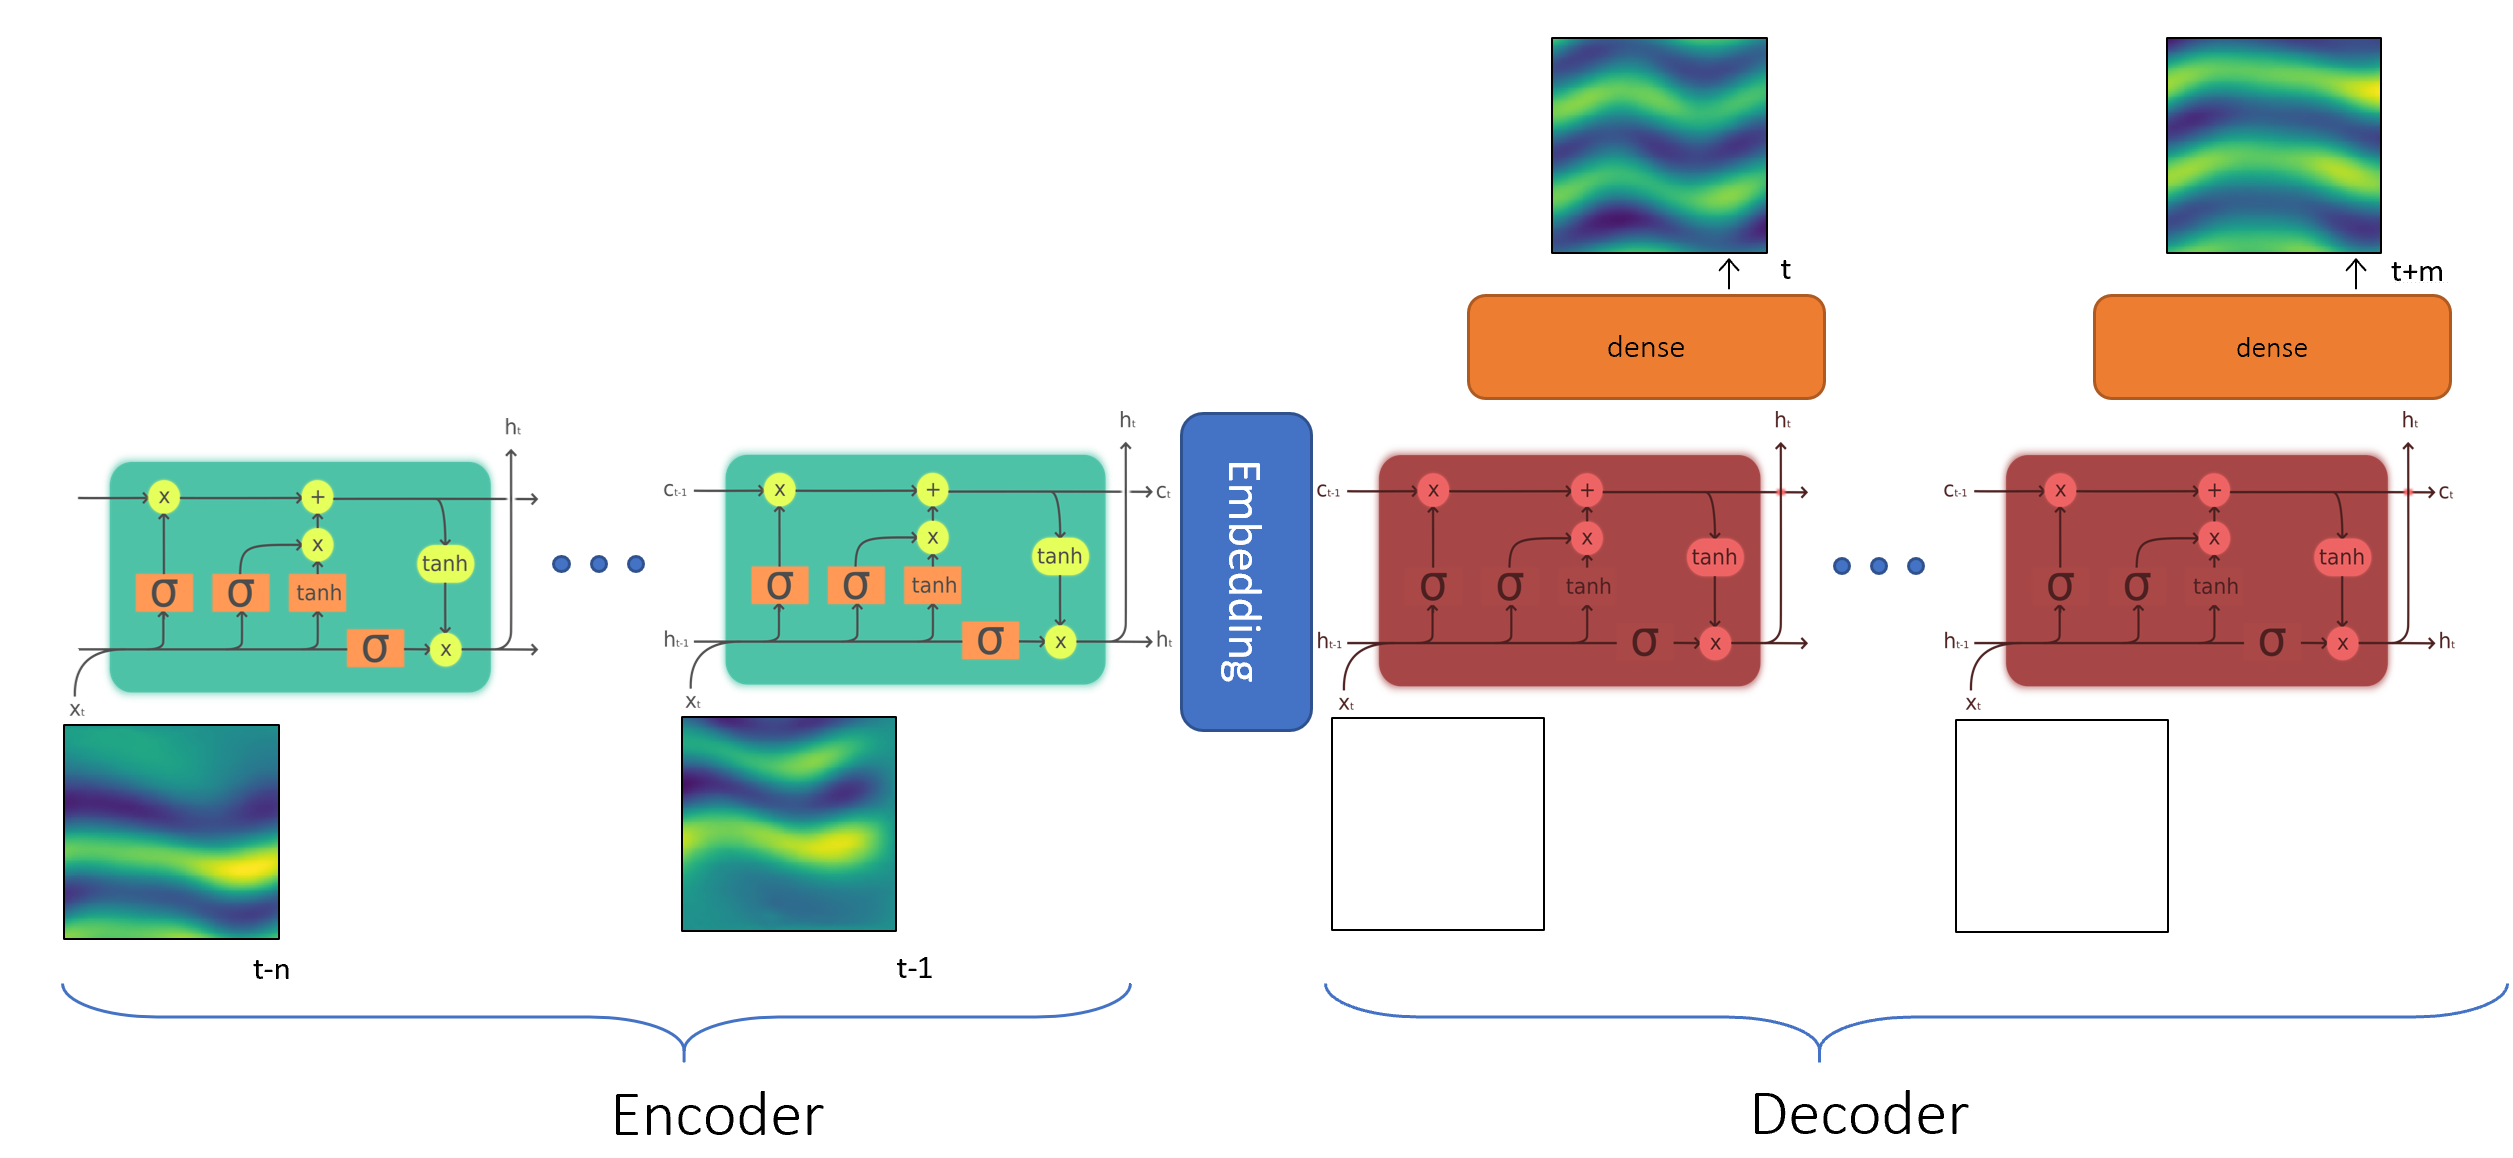
\includegraphics[width=0.8\textwidth]{images/lstm_setup.PNG}
		\caption{\small Illustration of encoder/decoder formulation 2 using separate long short term memory (LSTM) recurrent layers for the encoder and decoder with an additional linear activation layer (dense) to map the LSTM output to a vorticity image patch. For experiments in figure \ref{performance},  $n=20$ and $m=20$}
		\label{lstm_network_1}
	\end{center}	
\end{figure}

\begin{figure}
	\begin{center}
		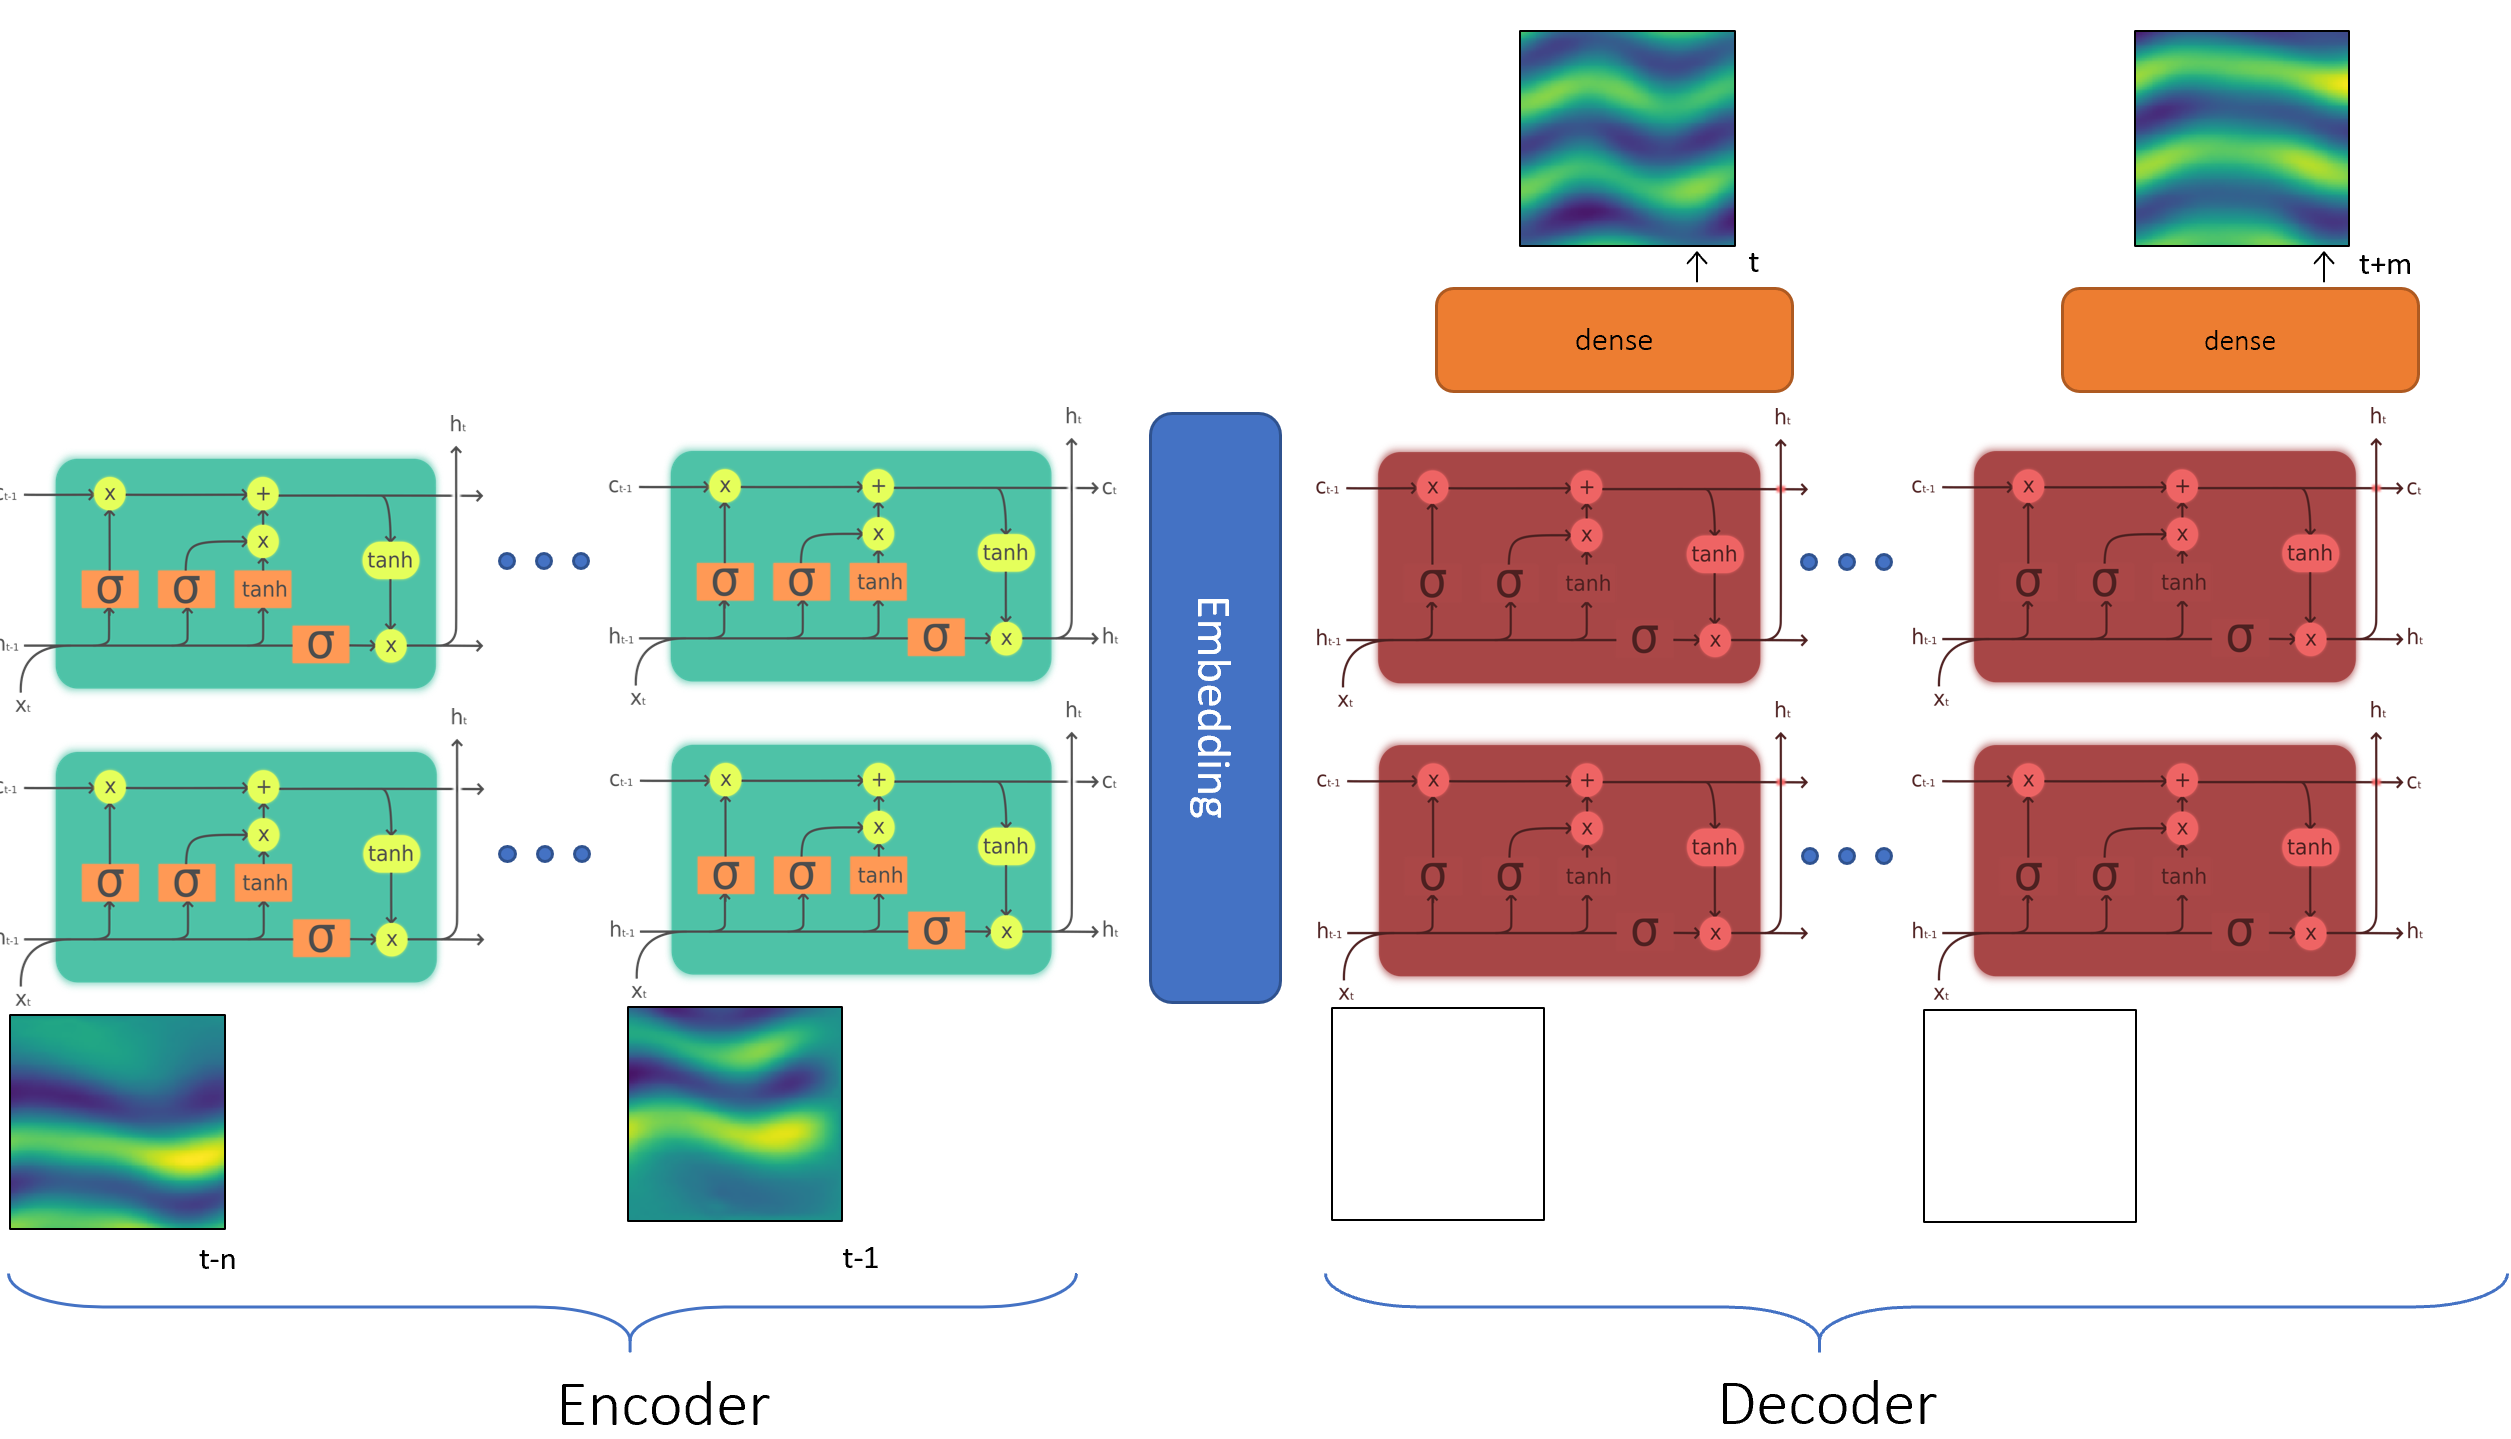
\includegraphics[width=0.78\textwidth]{images/lstm_2_setup.PNG}
		\caption{\small Illustration of encoder/decoder formulation 1, 3, and 4. This fomulation uses two stacked long short term memory (LSTM) recurrent layers for each the encoder and decoder with an additional linear activation layer (dense) to map the LSTM output to a vorticity image patch. Here $n=20$ and $m=20,200$}
		\label{lstm_network_2}
	\end{center}	
\end{figure}

Let $P_t \in \mathbb{R}^{360*279} $ be the turbulent flow at time $t \in \{1, 2, ..., 1000\}$ and define a window $w_{(r, t)}$ of $P_t$ in terms of a 50px by 50px region $r \in \{(u,v) \mid u \in \{0, ..., 309\}, v \in \{0, ...,  228\}\}$ 
For a particular region and time $(r,t) \in (\mathbb{R}^2,\mathbb{R})$ the input $x$ is a series of windows in the past, given by:
$$x = \{w_{(r,i)} \mid t-20 \leq i \leq t-1 \} \in \mathbb{R}^{50*50*20}$$ and our target $y$ is a single window of the form: $$y = \{w_{(r,i)} \mid i = t  \} \in \mathbb{R}^{50*50}$$


To train the network we randomly sample 50000 region, time pairs $S_i = \{(r, t) \mid i \in \{0, 1, ..., 4999\} \}$ and withhold 500 for validation creating two datasets, $X_{val} = \{w_{(S_i)} \mid i < 500 \} $ and $X_{train} = \{ {w_{(S_i)}\mid i \geq 500} \}$. We then learn a convolutional network $f(x)$ to minimize the Huber loss, $L(y, f(x))$ given by:
$$L(y, f(x)) = \begin{cases}
\max(0, 1 - y \, f(x))^2 & \textrm{for }\, \,  y \, f(x) \ge -1, \\
-4y \, f(x)              & \textrm{otherwise.}
\end{cases}$$

A network $f(x)$ is composed of a decoder and encoder network. Recurrent layers, namely long short term memory units (LSTM) are stacked to encode and decode an embedding of the input window shown in figures \ref{lstm_network_1} and  \ref{lstm_network_2}. Additionally, some networks utilize a dense layer representing a matrix multiplication of the output of the LSTM layer. This maps the output of the recurrent module to a single target $y$. Training is conducted over \num{1e+6} batches of 64 input - label sequences using the TensorFlow back-end and Adam optimizer.




\begin{figure}
	\begin{center}
		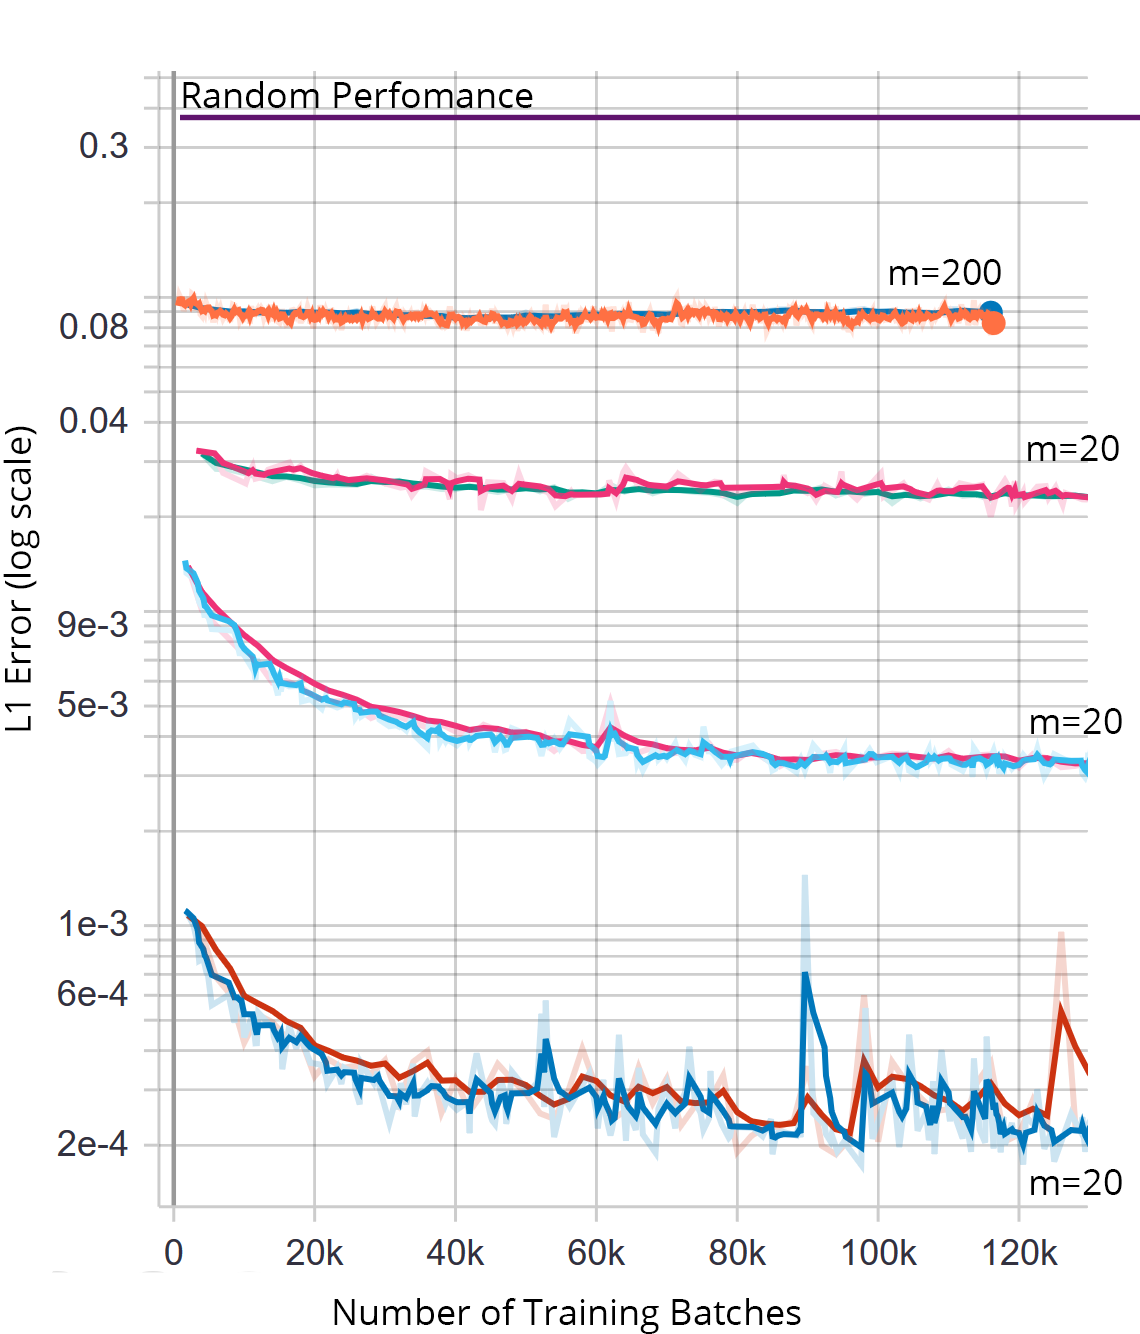
\includegraphics[width=0.7\textwidth]{images/acc_lstm.PNG}
		\caption{\small Comparison between four different networks and random performance, labeled top to bottom, random, network 1, 2, 3, and 4. Networks 2,3, and 4 are predict $m=20$ time-steps of vorticity. Network 2 uses a single LSTM layer for encoding and decoding as shown in figure \ref{lstm_network_1}. Network 3 adds an additional LSTM layer during encoding and decoding, as illustrated in figure \ref{lstm_network_2}. Network 4 uses same formulation as network 3, but utilizes an increased embedding size. Network 1 uses the best parameters found when training network 4, but attempts to predict 200 time-steps of vorticity, performing noticeably worse than any network predicting only 20 time-steps.}
		\label{performance}
	\end{center}	
\end{figure}







% == TECHNICAL ISSUES
\section{Issues and concerns (new \& ongoing).}

None






%\bibliographystyle{plain}
%\bibliography{}

\end{document}
